\documentclass[conference]{IEEEtran}

\usepackage{cite}
\usepackage{xcolor}
\usepackage{hyperref}
\hypersetup{colorlinks=true,linkcolor=black,citecolor=blue,filecolor=black,urlcolor=blue}
\usepackage{graphicx}
\graphicspath{{figures}}
\usepackage{caption}
\usepackage{subcaption}
\captionsetup[subfigure]{singlelinecheck=false, skip=0pt}
\usepackage{listings}
\renewcommand{\lstlistingname}{Algorithm}
\usepackage[binary-units=true]{siunitx}
\usepackage{csvsimple}
\usepackage{booktabs}

\newcommand{\TG}[1]{\color{blue}\textsc{From Tristan: }#1\color{black}}
\newcommand{\MD}[1]{\color{magenta}\textsc{From Mathieu: }#1\color{black}}
\newcommand{\HL}[1]{\hl{#1}}

\title{A Detailed Analysis of Performance Bottlenecks in MRI Pre-Processing}


\author{Mathieu Dugr\'e, Tristan Glatard \TG{I think Yohan should be co-author given his technical input}}

\begin{document}

\maketitle

\begin{abstract}
	% TODO																
\end{abstract}

\section{Introduction}
% Intro: Large dataset, long processing time, I/O intensive (derivatives), focus on MRI, no current study, pipelines?
% **Main question:** What are the main bottleneck in MRI pre-processing?
% **Why:** Performance of neuroimaging pipeline is critical (larger study, clinical use). However, limited study on performance profile.

\TG{Good intro but I think it would deserve a better logic. You could start by explaining that computational bottlenecks 
have been one of the main bottlenecks to the processing of large cohorts in neuroimaging, that the community is constantly searching for ways to process data faster (HPC, cloud, GPUs, DL models), and that your paper takes a step back by analyzing the computational bottlenecks in order to subsequently focus on their optimization. 
}

Magnetic Resonance Imaging (MRI) is a standard tool used by neuroscientists to perform clinical diagnosis and for researchers to develop a better understanding of the brain. Three main MRI techniques exist: structural MRI (sMRI), functional MRI (fMRI), and diffusion MRI (dMRI). While other modalities such as EEG, CT, and PET exist \TG{define acronyms}, we focus on MRIs for their broad adoption and non-invasive property. However, MRI data analysis is challenging due to computationally expensive pre-processing and large output and intermediate data size.

Neuroscientists developed various toolboxes to tackle the challenging task of pre-processing MRI data. Among those, some openly available and commonly accepted emerged: AFNI~\cite{Cox1996-sl}, ANTs~\cite{Avants_undated-fu}, FreeSurfer~\cite{Fischl2012-bp}, FSL~\cite{Jenkinson2012-cq}, and SPM~\cite{Friston2007-ag}. While the previous pipelines focus on specific steps of MRI pre-processing, tools like fMRIPrep~\cite{Esteban2019-og} and dMRIPrep~\cite{Michael2021-4515513} combine various pipelines to produce a complete pre-processing workflow.

The MRI pre-processing of a subject can take several hours, preventing the clinical use where data analysis might be required in timely manner. Moreover, the lengthy pre-processing hinders researchers with limited computational resources to perform research on large cohorts.

The first step to improve performance of an application is to understand its performance bottleneck. Following, we can focus our efforts on the performance critical components. For example, better algorithm designs or usage of hardware accelerator can reduce computation time. Compression techniques can lower data transfer time for output and intermediate data. At last, reduced precision arithmetic can lower computation time, memory footprint, and storage size. While these techniques can provide significant performance improvements, their implementation can require substantial effort. Therefore, it is critical to understand the performance bottleneck of MRI pre-processing pipelines to improve their performance.

The neuroimaging community is well aware that MRI pre-precessing pipelines require long computation time. However, to the best of our knowledge, there is no comprehensive study of the performance bottlenecks in MRI pre-processing. In this paper, we characterize computational cost of several commonly adopted MRI pre-processing pipelines. The results of our analysis serve as a reference for future efforts to optimize MRI pre-processing workflows.

\TG{you could summarize the method (vtune profiler) in the intro.}

\section{Methods}
\subsection{Infrastructure}
For our experiments, we used the \textit{Slashbin cluster} at Concordia University. The cluster has eight compute nodes, each configured with two 16-core Intel(R) Xeon(R) Gold 6130 CPU @ \SI{2.10}{\giga\hertz}, \SI{250}{\gibi\byte} of RAM, \SI{126}{\gibi\byte} of tmpfs, six \SI{447}{\gibi\byte} SSDs with the XFS file system (no RAID enabled), CentOS~8.1 and Linux kernel \textit{4.18.0-477.10.1.el8\_lustre.x86\_64}. \TG{I would defer this subsection to later in the methods as it's not the most central one}

\subsection{Data}
To ensure the performance profiles of the applications derived from our work are inclusive of different populations, we used data with a wide range of age and equal distribution of sex (biological). Using a diverse dataset should help to prevent findings of potential performance bottleneck associated to a specific population.

We used the the OpenNeuro ds004513 v.1.0.2 dataset~\cite{ds004513:1.0.2}. The anatomical, functional, and diffusion data from 20 health individuals was acquired from two different cohorts. The within-subject cohort has nine participants (mean age=43~yrs, std=7~yrs; 4 females) with two session: eyes open and eyes closed. The replication cohort has eleven participants (mean age=27~yrs, std=5~yrs; 6 females) with only the eyes open session. We profiled the application using both cohort on the eyes open session, unless explicitly specified.

\subsection{Pipelines}
% TODO rework
In this analysis, we aim to cover the pre-processing performance for different MRI modalities. We study the performance bottleneck of large toolboxes and individual pipelines. Moreover, we use several pipelines from the LivingPark project~\cite{livingpark} as a real use case of MRI pre-processing.

First, we profile these commonly accepted workflows: fMRIPrep anatomical only without and without FreeSurfer, fMRIPrep complete workflow, and dMRIPrep. This lets us study the coarse grain performance of workflows for anatomical, functional, and diffusion MRI pre-processing.

Second, we perform a finer grain analysis of the aforementioned workflows' sub-components. We list the different sub-workflow and describe the key steps for each modality in the section below.

Last, the LivingPark project replicates several papers on Parkinson's Disease with a broad range of analysis. The study uses the following pipelines: FSL SIENA/VIENA, SPM VBM, SPM DARTEL, and SPM pairwise registration.
% TODO Decide which pipelines to use from the project.

% ############################################################
% Pre-Processing
% ############################################################
% Look at the benchmarked tool and the information needed to abstract those tools.
% Discussion of the pre-processing steps.
% Explain their computation and I/O requirements.
\subsection{sMRI Pre-Processing}
\subsubsection{Intensity correction}
% N4 bias correction (Check ANTS brainExtraction)
% https://ieeexplore.ieee.org/document/5445030

\subsubsection{Reference Image}
% Longitudinal study 
% FreeSurfer mri_robust_template

\subsubsection{Spatial Normalization}
% ANTS registrationSyN
% SyN Registration: https://pubmed.ncbi.nlm.nih.gov/17659998/


\subsubsection{Skull-Stripping}
% ANTS brainExtraction
% 1. Truncate image intensity
% 2. N4 bias correction
% 3. SyN Registration
% 4. Warp prior to image using affine
% 5. Atropos: https://pubmed.ncbi.nlm.nih.gov/21373993/


\subsubsection{Segmentation}
% FSL FAST


\subsubsection{Surface Reconstruction}
% FreeSurfer recon-all


\subsection{fMRI Pre-Processing}
\subsubsection{Slice-Timing Correction}
% AFNI 3dTShift


\subsubsection{Head-Motion Correction}
% FSL MCFLIRT


\subsubsection{Susceptibility Distortion Correction}
% SDC workflow


\subsubsection{Registration}
% FSL FLIRT


\subsection{dMRI Pre-Processing}
% TODO: Decide which pipelines to use
% \subsubsection{Eddy Currents Distortion Estimation}
% % FSL eddy


\subsection{Profiling}
Profiling MRI pre-processing pipelines present a set of challenges. The neuroimaging community develops pipelines using several programming languages including \textit{C}, \textit{C++}, \textit{Fortran}, \textit{Python}, and \textit{Matlab}, with several pipelines utilizing a combination of multiple languages. Pipelines are generally complex and computationally expensive.

The Intel VTune profiler~\cite{vtune_profiler} satisfies these challenges by offering multi-language support, low performance overhead, and information of functions at runtime level. However, ome general profiling challenges remain. Profilers require source code to be compiled with Debug Symbols to report useful information about the different functions and modules. Moreover, different input data can substantially vary the analysis due to conditional branching in the application and convergence thresholds. We discuss our approach to these challenges in the next section.
% TODO add citation on effect of different input data on numerical stability and reduced precision.

First, to obtain human readable information on function and module names in VTune, we re-compiled each pipeline with debug information in a Docker image. For use on HPC systems, we created Singularity images using Docker2Singularity \lstlistingname~\ref{vtune_example} illustrate the profiling of a pipeline by mounting the VTune binary to the Singularity image at execution.
\lstinputlisting[
	language={sh},
	caption={Profiling an application within a Singularity container, using VTune profiler.},
	captionpos=b,
	label=vtune_example,
	numbers=left,
	frame=single,
	basicstyle=\footnotesize,
	numbersep=5pt,
	numberstyle=\tiny\color{gray},
	rulecolor=\color{black},
	tabsize=2,
]{vtune-example.sh}

Second, to estimate an average performance profile, we aggregate the profiling results of each pipeline across all subjects. Combining the Pareto's law and VTune hotspots report \TG{It would be useful to define these terms}, we present the functions accounting for most of the CPU time up to 80\% of the total CPU time of the application \TG{check wording}. This heuristic allows us to focus our efforts on the performance critical sections of a pipeline. We report the mean and standard deviation of the execution time for those functions.

Last, we profile the application two threading configuration: single-threaded and 32 threads. On the one hand, the single-threaded approach limits the potential overhead from I/O on the profiling. On the other hand, we evaluate the multi-threading performance of the applications using maximum number of CPU core available on our system (i.e. 32).

Before profiling each application, we transfer the input data from the shared file system to the compute node. After profiling, we transfer back the output to the shared file system. This limits profiling variability due to I/O contingency.

The data generated by the VTune profiler is written to a shared file system, for administrative reasons. Theoretically, this increase the profiling overhead. However, in practice there is no impact since the data generated by the VTune profiler is very small and is not written on the same file system as the data from applications.

\section{Results}
\TG{Interesting results but presentation needs to be worked out. This section should be structured with sub-headings summarizing the main findings, for instance: "Interpolation is the main bottleneck", etc}

% TODO
% 2-step approach:
% 1. Which pipeline constitute the long execution time in preprocessing?
% 2. For those, which functions take the most time to execute? (hotspots)
% Any key finding: common point between functions, mem bound, fops, etc.

% In this section, analyze the aggregated profiling data obtained with VTune. First, a coarse summary of the workflows and pipelines is presented using their makespan. Second, we depict detailed analysis for the key functions contributing to the CPU time of each application (hotspots).

\subsection{Makespan}
% Identify which tools take the longest to execute.
% This will let us decided which pipeline to investigate more.
Figure~\ref{fig:makespan-1thread} shows the mean and standard deviation of the makespan \TG{define makespan}, in seconds, while using 1 thread for one execution of all subjects.
Unexpectedly, we observe that both ANTS~BrainExtration and ANTS~RegistrationSyN are slower when using single precision compared to double precision.
% TODO Stat test between mean for single and double precision.
\begin{figure}[h]
	\centering
	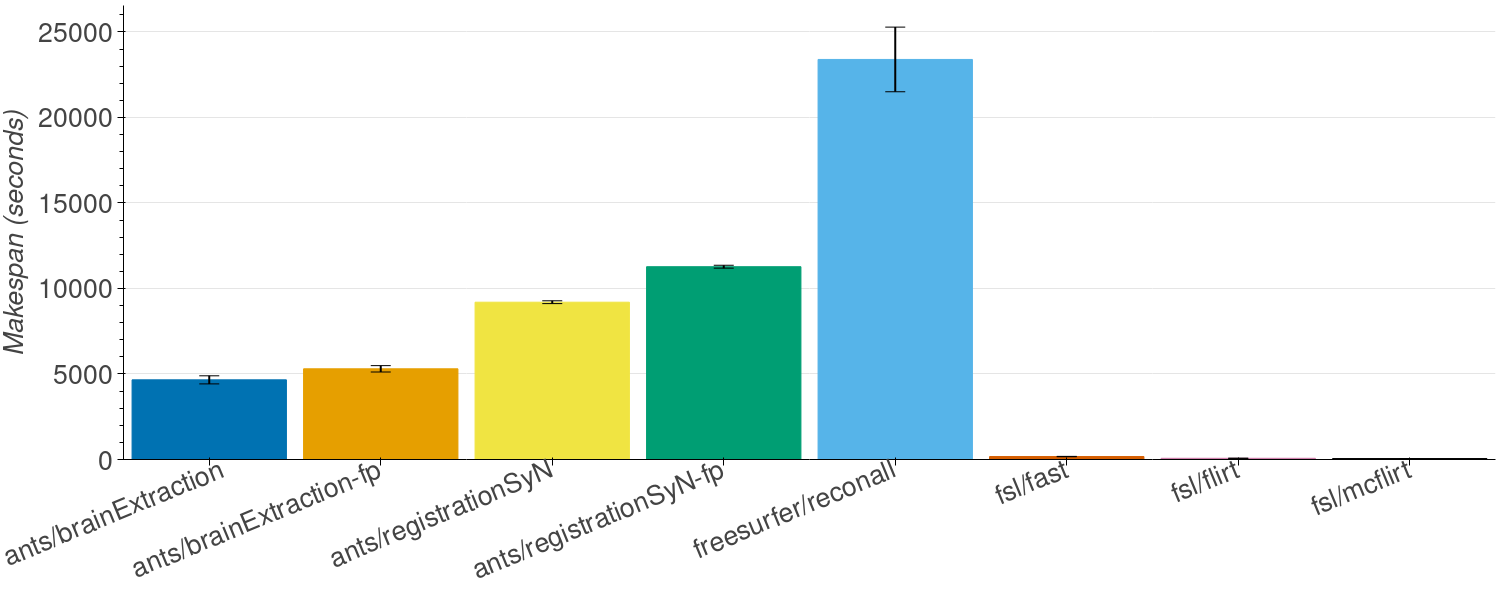
\includegraphics[width=\linewidth]{figures/makespan-1thread.png}
	\caption{Profiling of the pipelines using 1 thread. \TG{Font size in the figure is too small, it should be similar to the caption font size}}
	\label{fig:makespan-1thread}
\end{figure}

\subsection{Hotspots}

Figure~\ref{fig:hotspots-fmriprep-anat-subworkflow} depicts the hotspots observed from profiling the fMRIPrep anatomical sub-workflows. In each sub-figure, the x-axis shows the function ID grouped by parent module, which are ordered by CPU time of (1) the modules, then (2) the functions within a module. The function ID are found in the supplementary material Section~\ref{sec:supplementary}. The bars show the average CPU time in seconds of a function and the error bars indicate the standard deviation, with the left y-axis showing the scale. The light-green dots represent the functions cumulative percentage makespan of the application, with the right y-axis showing the scale. The color of the bar indicate the percentage of calls, for the function, that were ``stalled due to demand memory loads and stores''\footnote{\href{https://www.intel.com/content/www/us/en/docs/vtune-profiler/user-guide/2023-0/cpu-metrics-reference.html\#MEMORY-BOUND}{Vtune Memory Bound metric}}, with the left color bar showing the scale.

\TG{I'd move the graphical explanations to the figure caption so that the text can focus on observations}

In figure~\ref{subfig:hotspots-ants-brainExtraction}, we observe that the function 1 and 2 account for a significant portion of the application execution time. Moreover, calls from function~1 are memory bound $51.84\pm{4.55}$ percent of the time. Table~\ref{extab:hotspots-1thread-ants-brainExtraction} shows that both functions are part of the ITK linear interpolation module.

Similarly, figure~\ref{subfig:hotspots-ants-brainExtraction-fp} shows the same two functions accounting for the most time, although in flipped order. Calls from function~2 are memory bound $36.30\pm{4.98}$ percent of the time. Compared to the double precision version of ANTS brainExtraction, the third function runtime is significantly larger. It is an ITK function transforming points while calculating the displacement field of the image.

Figure~\ref{subfig:hotspots-ants-registrationSyN} and figure~\ref{subfig:hotspots-ants-registrationSyN-fp} show that the execution time for ANTS registrationSyN is dominated by a single function. In both case, the ITK function evaluating point during linear interpolation. The next two function are also shared between the application, although in flipped order. These functions show some memory bound in the range of 16--27.5. We also note the three most expensive functions are the same as in both versions of ANTS brainExtraction.

% TODO FreeSurfer 1-thread sub-figure

In figure~\ref{subfig:hotspots-32threads-freesurfer-reconall}, we observe that OMP is a major bottleneck for the application, accounting for at least 76\% of the application runtime. The only function shown from FreeSurfer recon-all is the same as the first function from figure~\ref{subfig:hotspots-1thread-freesurfer-reconall}. However, it only accounts for 2\% of the total makespan compared to 3.8\% while running sequentially.

\begin{figure*}[ht!]
	\centering
	% ANTS brainExtraction
	\begin{subfigure}[t]{0.49\textwidth}
		\caption{}
		\label{subfig:hotspots-ants-brainExtraction}
		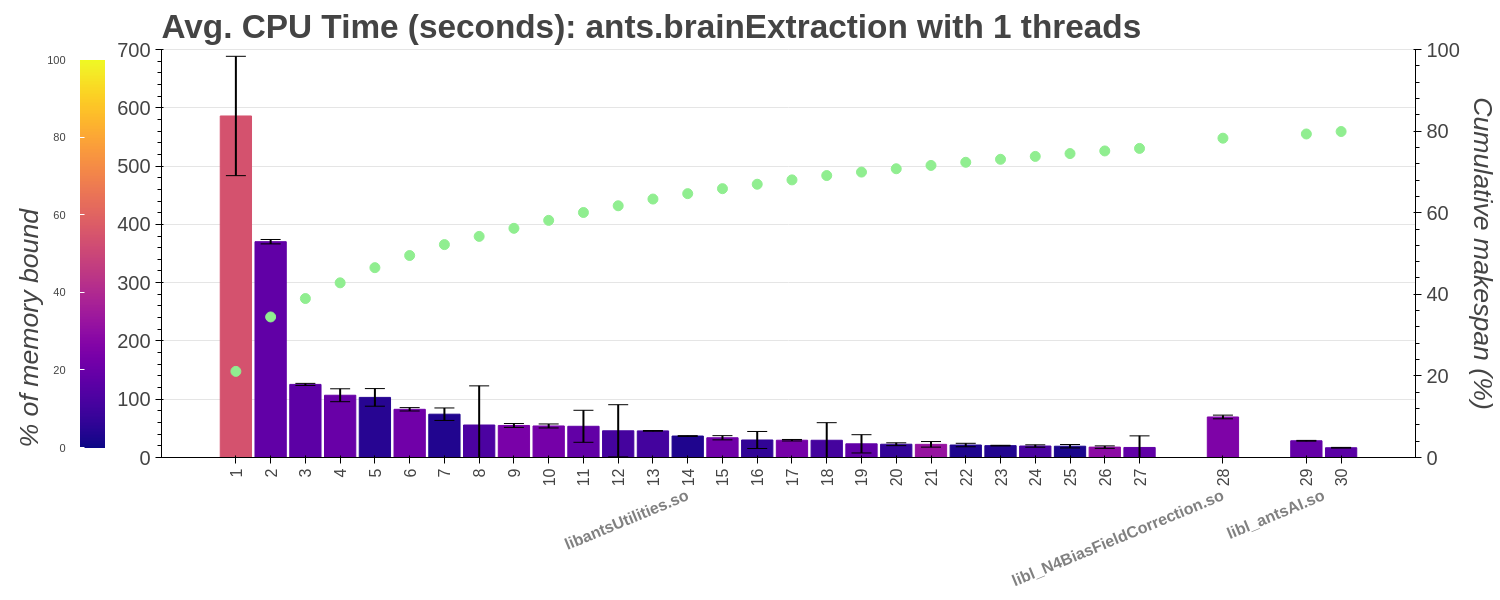
\includegraphics[width=\textwidth]{figures/hotspots-1thread-ants-brainExtraction.png}
	\end{subfigure}
	\hfill
	\begin{subfigure}[t]{0.49\textwidth}
		\caption{}
		\label{subfig:hotspots-ants-brainExtraction-fp}
		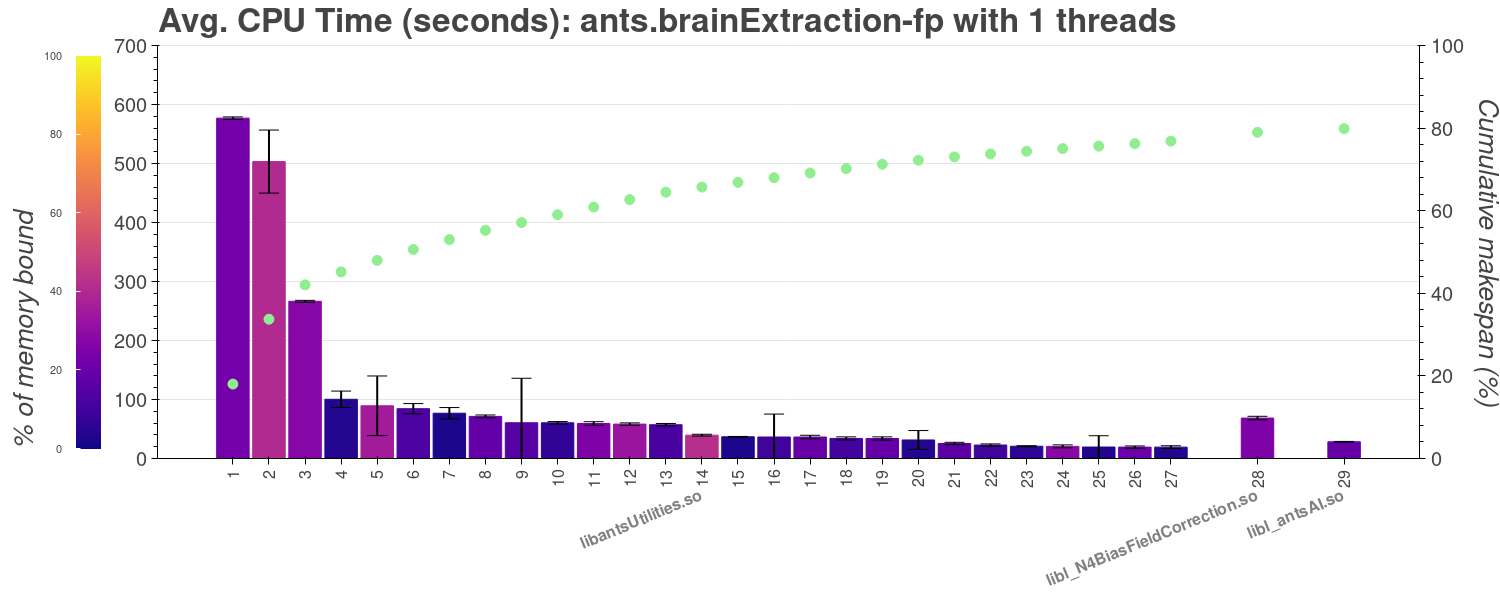
\includegraphics[width=\textwidth]{figures/hotspots-1thread-ants-brainExtraction-fp.png}
	\end{subfigure}
	% ANTS registrationSyN
	\begin{subfigure}[t]{0.49\textwidth}
		\caption{}
		\label{subfig:hotspots-ants-registrationSyN}
		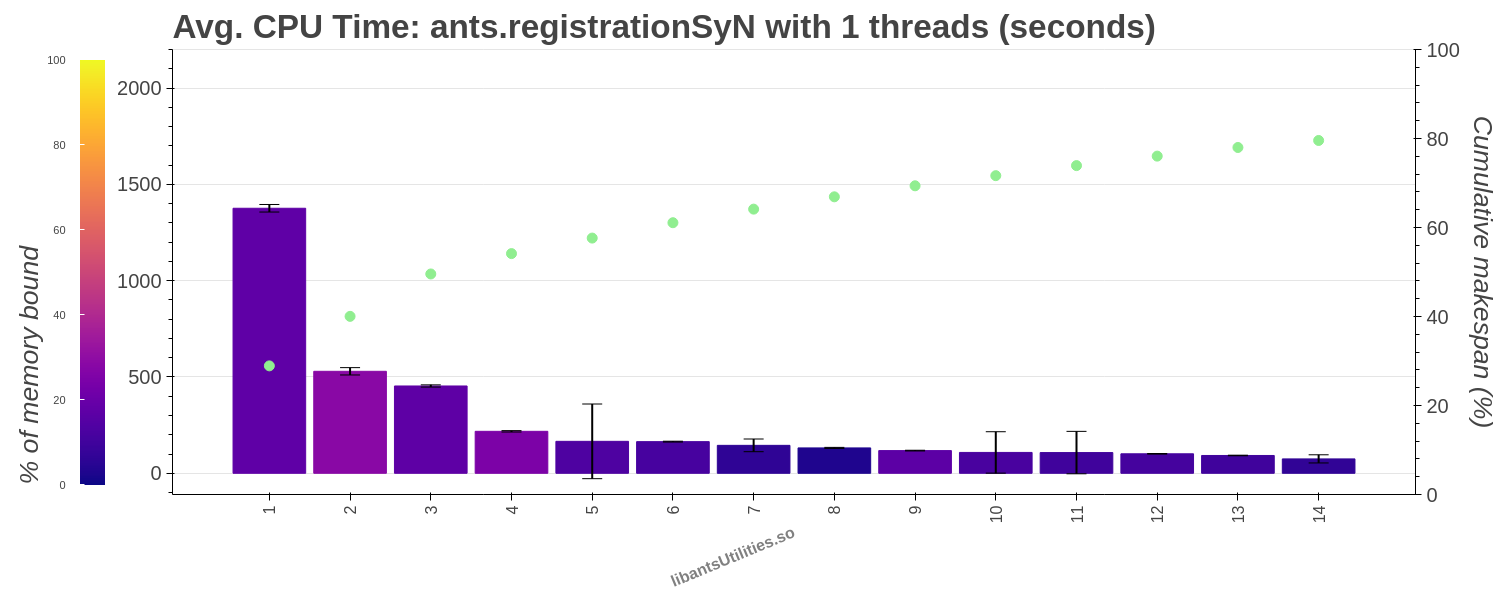
\includegraphics[width=\textwidth]{figures/hotspots-1thread-ants-registrationSyN.png}
	\end{subfigure}
	\hfill
	\begin{subfigure}[t]{0.49\textwidth}
		\caption{}
		\label{subfig:hotspots-ants-registrationSyN-fp}
		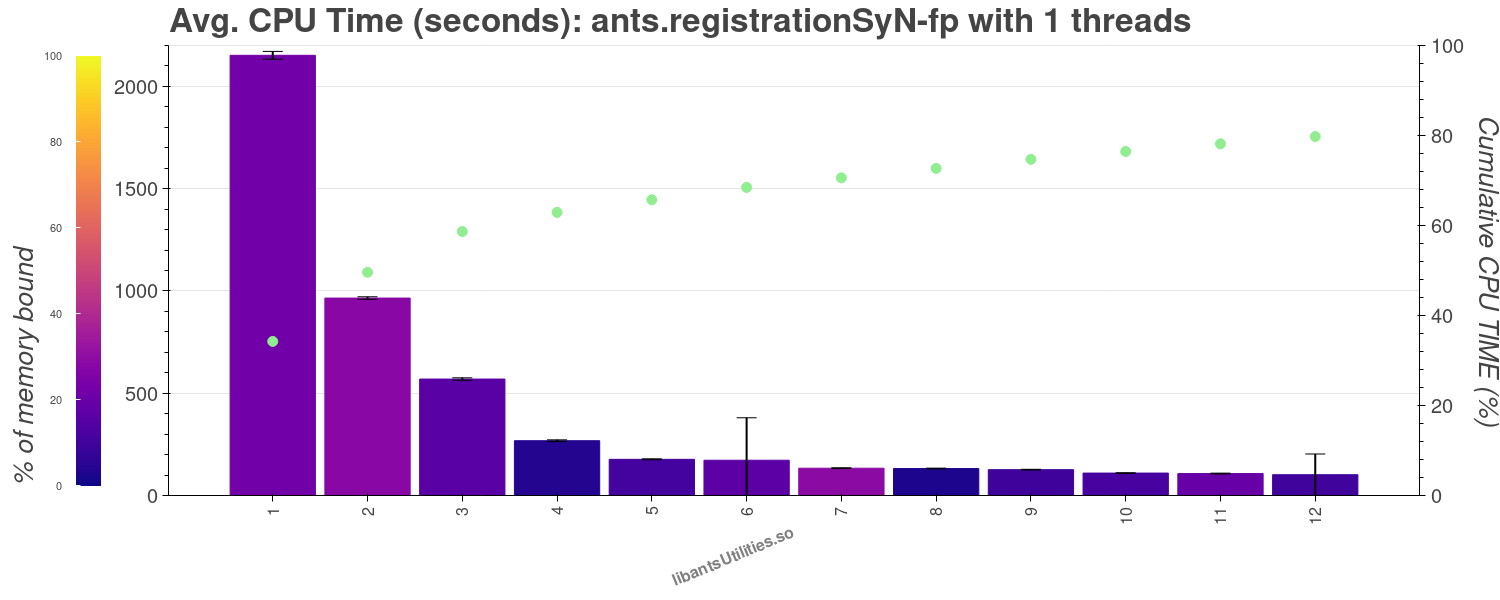
\includegraphics[width=\textwidth]{figures/hotspots-1thread-ants-registrationSyN-fp.png}
	\end{subfigure}
	\caption{ANTS: Single vs. Double precision}
	\label{fig:ants-fp-comparison}
\end{figure*}
					
\section{old Results}
% TODO
% 2-step approach:
% 1. Which pipeline constitute the long execution time in preprocessing?
% 2. For those, which functions take the most time to execute? (hotspots)
% Any key finding: common point between functions, mem bound, fops, etc.
					
% In this section, analyze the aggregated profiling data obtained with VTune. First, a coarse summary of the workflows and pipelines is presented using their makespan. Second, we depict detailed analysis for the key functions contributing to the CPU time of each application (hotspots).
		
					
\subsection{Hotspots}
Figure~\ref{fig:hotspots-fmriprep-anat-subworkflow} depicts the hotspot observed from profiling the fMRIPrep anatomical sub-workflows. In each sub-figure, the x-axis shows the function ID grouped by parent module, which are ordered by CPU time of (1) the modules, then (2) the functions within a module. The function ID are found in the supplementary material Section~\ref{sec:supplementary}. The bars show the average CPU time in seconds of a function and the error bars indicate the standard deviation, with the left y-axis showing the scale. The light-green dots represent the functions cumulative percentage makespan of the application, with the right y-axis showing the scale. The color of the bar indicate the percentage of calls, for the function, that were ``stalled due to demand memory loads and stores''\footnote{\href{https://www.intel.com/content/www/us/en/docs/vtune-profiler/user-guide/2023-0/cpu-metrics-reference.html\#MEMORY-BOUND}{Vtune Memory Bound metric}}, with the left color bar showing the scale.
					
In figure~\ref{subfig:hotspots-ants-brainExtraction}, we observe that the function 1 and 2 account for a significant portion of the application execution time. Moreover, calls from function~1 are memory bound $51.84\pm{4.55}$ percent of the time. Table~\ref{extab:hotspots-1thread-ants-brainExtraction} shows that both functions are part of the ITK linear interpolation module.
					
Similarly, figure~\ref{subfig:hotspots-ants-brainExtraction-fp} shows the same two function accounting for the most time, although in flipped order. Calls from function~2 are memory bound $36.30\pm{4.98}$ percent of the time. Compared to the double precision version of ANTS brainExtraction, the third function runtime is significantly larger. It is an ITK function transforming points while calculating the displacement field of the image.
					
Figure~\ref{subfig:hotspots-ants-registrationSyN} and figure~\ref{subfig:hotspots-ants-registrationSyN-fp} show that the execution time for ANTS registrationSyN is dominated by a single function. In both case, the ITK function evaluating point during linear interpolation. The next two function are also shared between the application, although in flipped order. These functions show some memory bound in the range of 16--27.5. We also note the three most expensive functions are the same as in both versions of ANTS brainExtraction.
					
% TODO FreeSurfer 1-thread sub-figure
% Note:
% - Way more functions
% - Top 5 accounts for only 15% of total time. Much less than other applications.
% - Way more memory bound that previous application.
% - Focusing on Top 5 and memory bound could give good performance boost.
					
\begin{figure*}[ht!]
	\centering
	% % ANTS brainExtraction
	% \begin{subfigure}[t]{0.49\textwidth}
	% 	\caption{}
	% 	\label{subfig:hotspots-ants-brainExtraction}
	% 	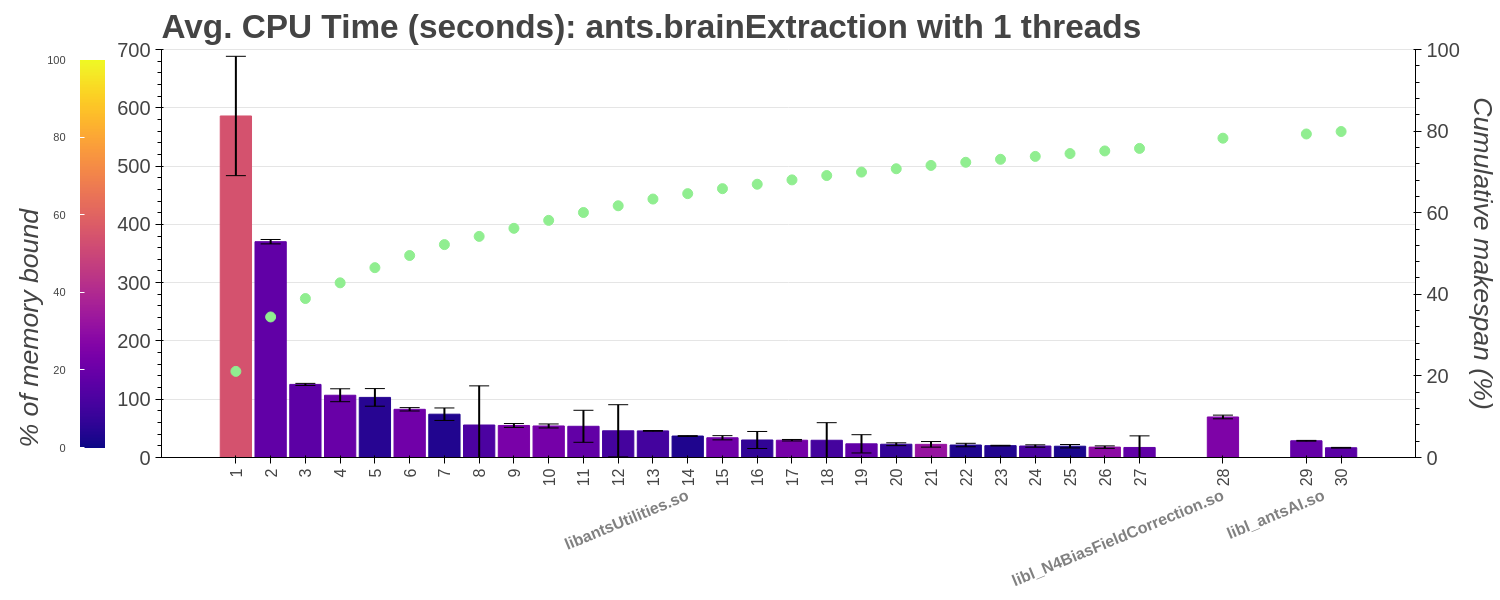
\includegraphics[width=\textwidth]{figures/hotspots-1thread-ants-brainExtraction.png}
	% \end{subfigure}
	% \hfill
	% \begin{subfigure}[t]{0.49\textwidth}
	% 	\caption{}
	% 	\label{subfig:hotspots-ants-brainExtraction-fp}
	% 	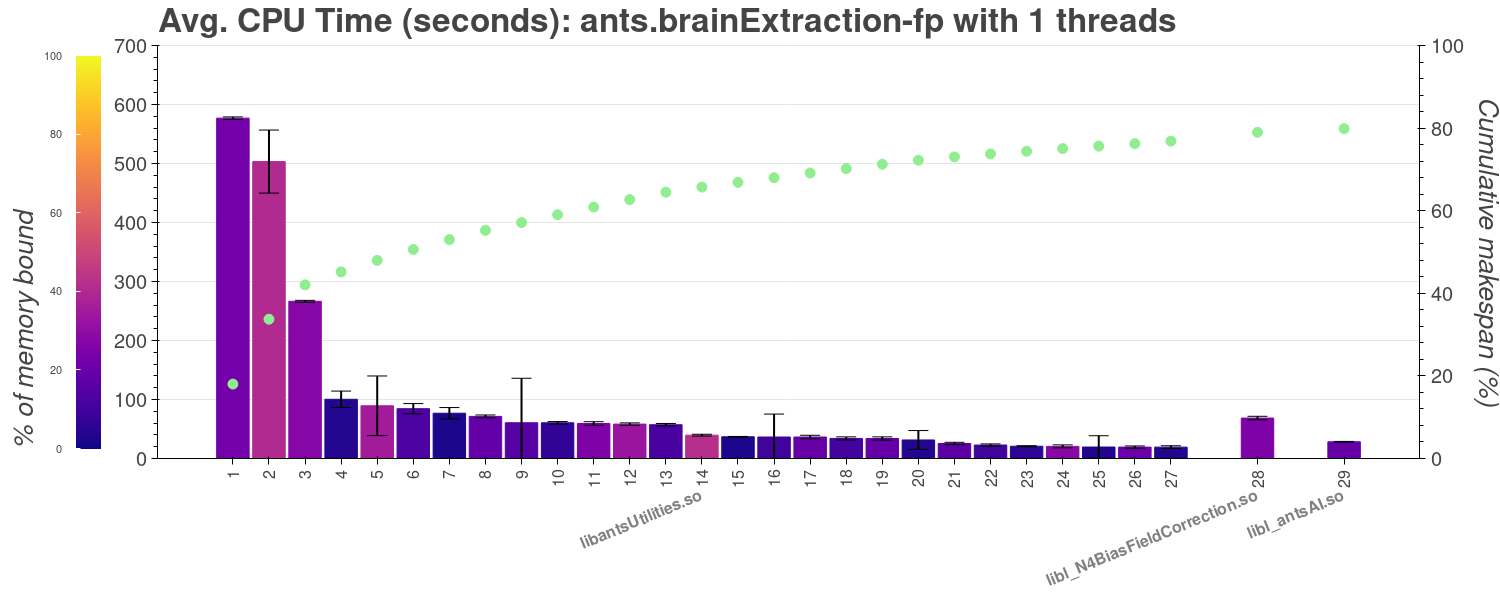
\includegraphics[width=\textwidth]{figures/hotspots-1thread-ants-brainExtraction-fp.png}
	% \end{subfigure}
																																																																																																															
	% % ANTS registrationSyN
	% \begin{subfigure}[t]{0.49\textwidth}
	% 	\caption{}
	% 	\label{subfig:hotspots-ants-registrationSyN}
	% 	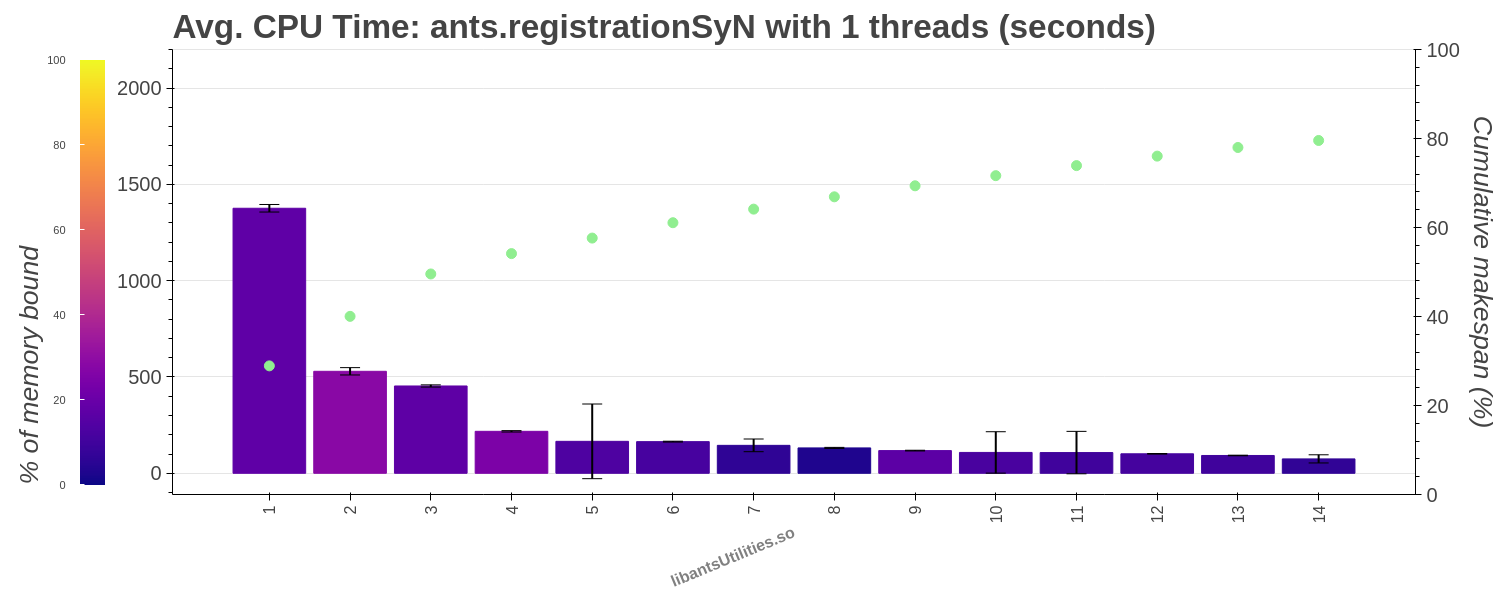
\includegraphics[width=\textwidth]{figures/hotspots-1thread-ants-registrationSyN.png}
	% \end{subfigure}
	% \hfill
	% \begin{subfigure}[t]{0.49\textwidth}
	% 	\caption{}
	% 	\label{subfig:hotspots-ants-registrationSyN-fp}
	% 	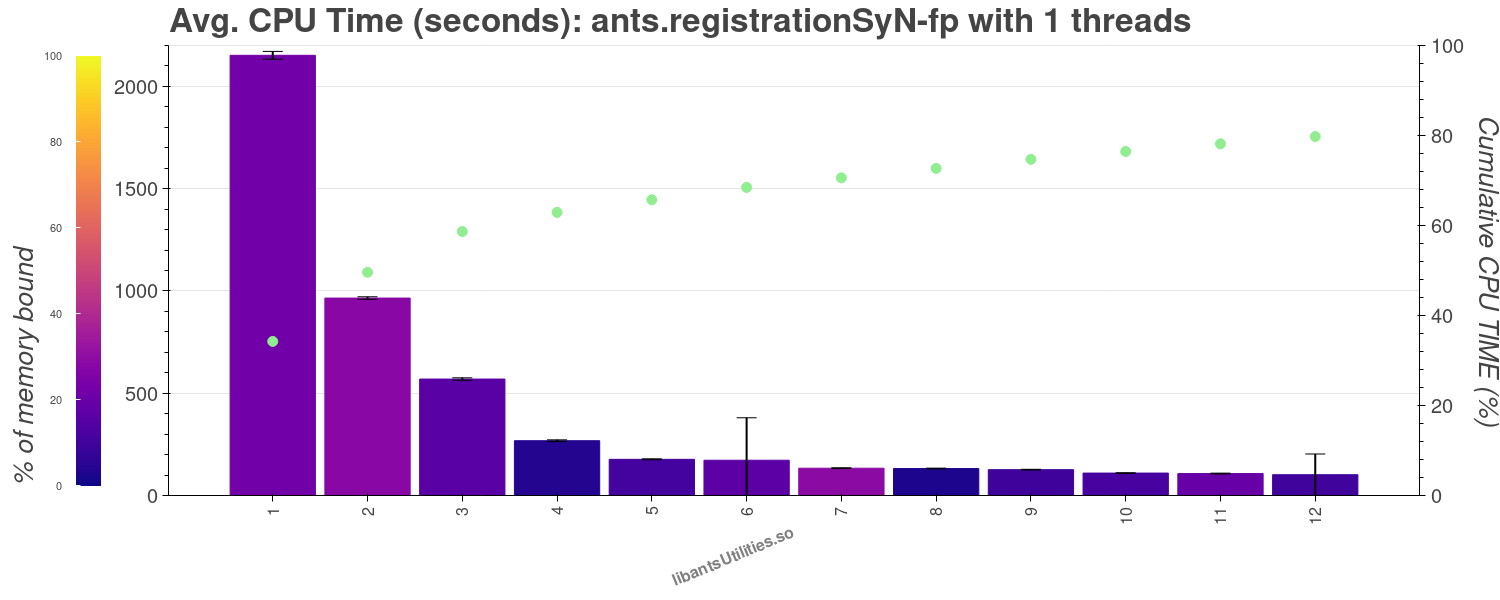
\includegraphics[width=\textwidth]{figures/hotspots-1thread-ants-registrationSyN-fp.png}
	% \end{subfigure}
																																																																																																															
	% % FreeSurfer recon-all
	% \begin{subfigure}[t]{\textwidth}
	% 	\caption{}
	% 	\label{subfig:hotspots-1thread-freesurfer-reconall}
	% 	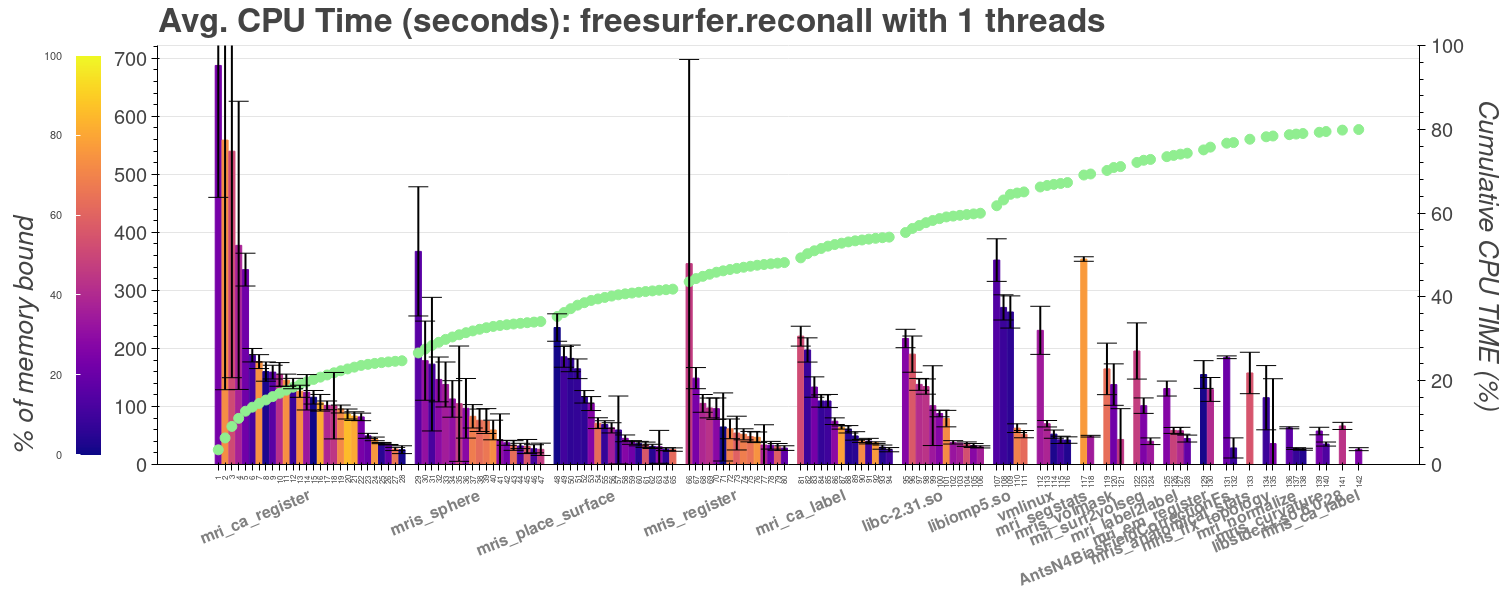
\includegraphics[width=\textwidth]{figures/hotspots-1thread-freesurfer-reconall.png}
	% \end{subfigure}
																																																																																																															
	% \begin{subfigure}[t]{0.49\textwidth}
	% 	\caption{}
	% 	\label{subfig:hotspots-32threads-freesurfer-reconall}
	% 	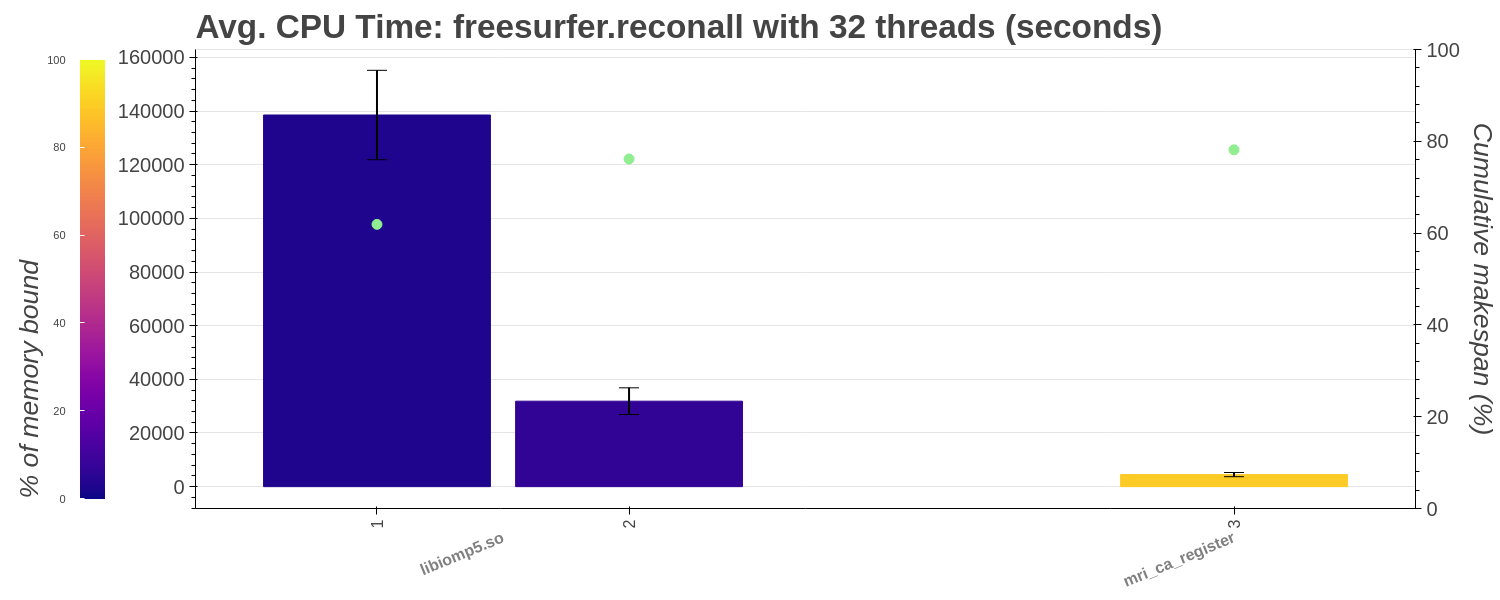
\includegraphics[width=\textwidth]{figures/hotspots-32threads-freesurfer-reconall.png}
	% \end{subfigure}
	\hfill
	% FSL FAST
	\begin{subfigure}[t]{0.49\textwidth}
		\caption{}
		\label{subfig:hotspots-fsl-fast}
		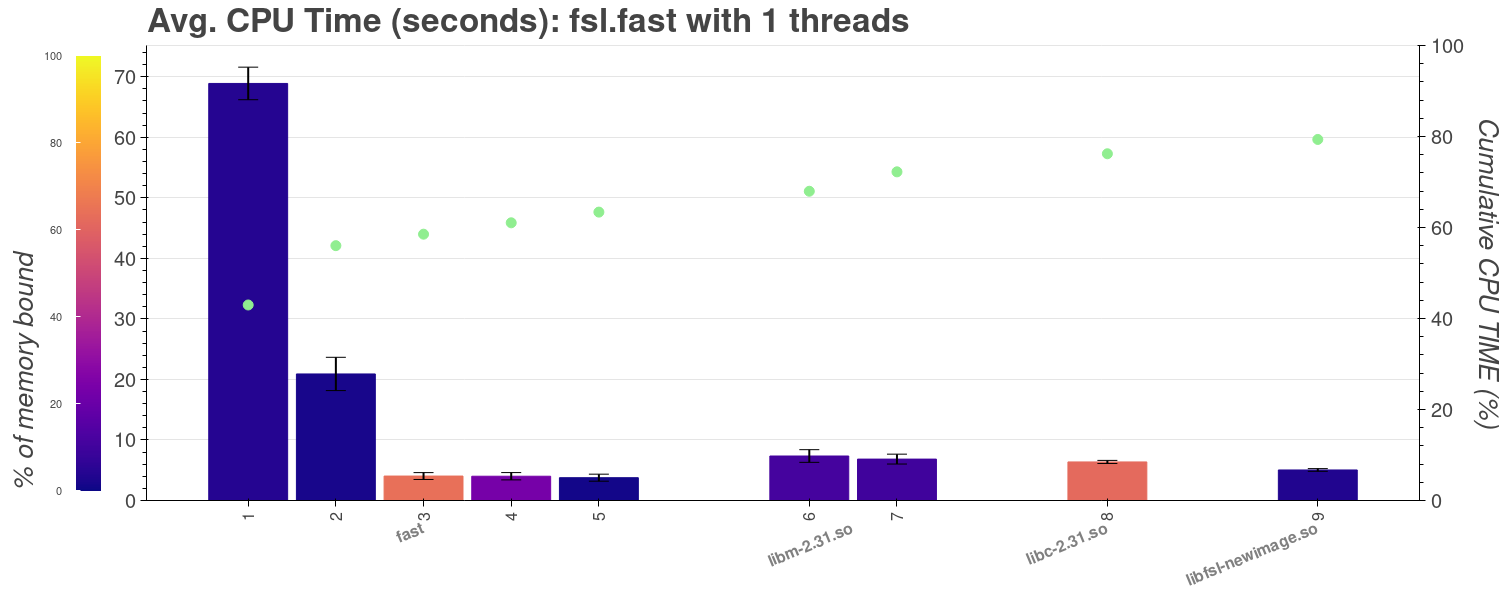
\includegraphics[width=\textwidth]{figures/hotspots-1thread-fsl-fast.png}
	\end{subfigure}

	\caption{Hotspots profiling of fMRIPrep's anatomical sub-workflows.}
	\label{fig:hotspots-fmriprep-anat-subworkflow}
	
	% TODO: Describe the plot components. Plots are quite complex so this will be necessary for proper understanding.
\end{figure*}
					
\begin{figure*}[ht!]
	\centering
	% FSL MCFLIRT
	\begin{subfigure}[t]{0.49\textwidth}
		\caption{}
		\label{subfig:hotspots-fsl-mcflirt}
		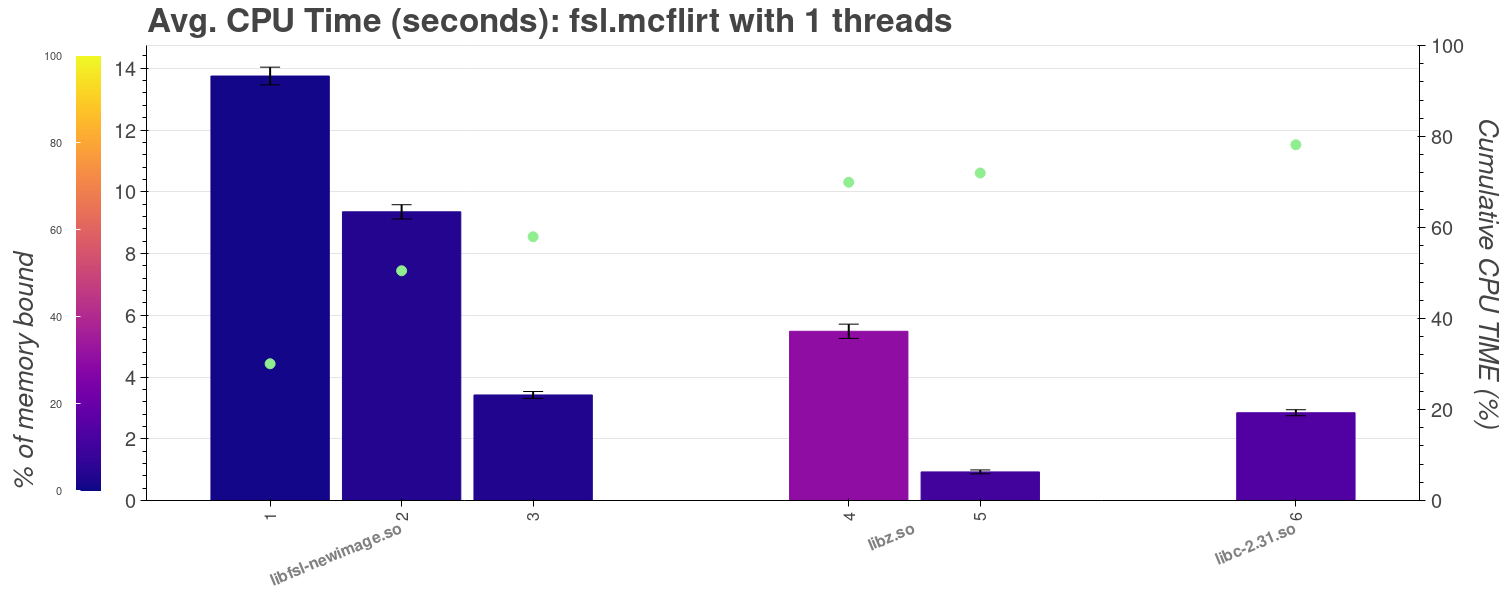
\includegraphics[width=\textwidth]{figures/hotspots-1thread-fsl-mcflirt.png}
	\end{subfigure}
	% FSL FLIRT
	\hfill
	\begin{subfigure}[t]{0.49\textwidth}
		\caption{}
		\label{subfig:hotspots-fsl-flirt}

		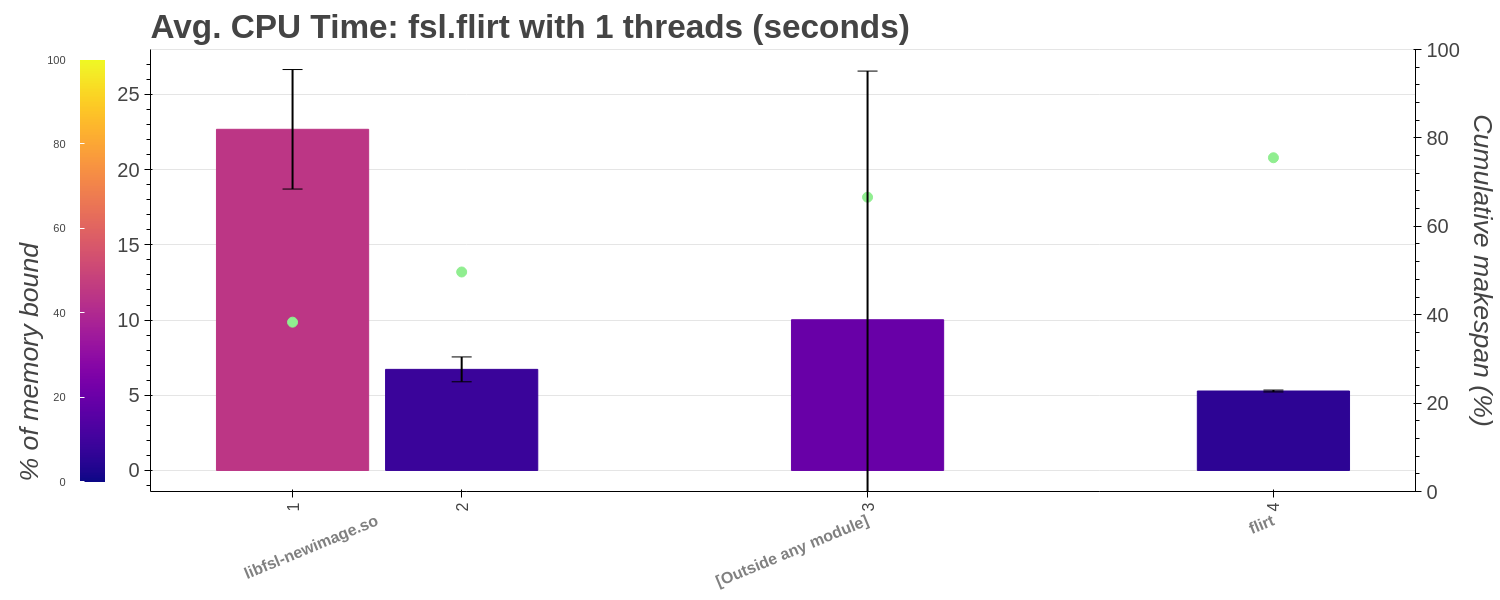
\includegraphics[width=\textwidth]{figures/hotspots-1thread-fsl-flirt.png}
	\end{subfigure}
	\caption{Hotspots profiling of fMRIPrep's functional sub-workflows.}
	\label{fig:hotspots-fmriprep-func-subworkflow}														
	
	% TODO: Describe the plot components. Plots are quite complex so this will be necessary for proper understanding.
\end{figure*}
					
\section{Discussion}
% TODO
					
% Principal Bottlenecks
% What are common key points between the different applications?
% Possibly move this to the Results section.
% - Top 3 functions in ANTS application are the same, although in varying order.
% - 
					
% # Limitation
% - Can only perform profiling of open-source pipelines or pipelines with debug-info.
% - No information about space or time for function call.
% - Dataset only contains healthy subjects (no pathology).
% - Dataset is from a single site. Possible bias from scanner or protocol.
					
% # Opportunity for optimization (future work)
% Reduced precision for: Compute or Compression. Reduce memory footprint and compute time. -> Mention the applications with high FP-ops and MEM-bound.
					
% # Linear Interpolation
% Theoretical improvements using reduced precision. If time permits, toy experiment with ITK single precision data type at different locations.
					
% # Single precision slowdown?
% Possibly due to slower convergence and less optimized code. (Quick drop-in of ITK single precision data type.)
% Need to investigate more.
					
% OpenOMP bottleneck (FreeSurfer with 32 threads)
% Majority of the time is spent waiting to synchronize threads.
% If times permit, changes the scheduling type and run for a subject to see if we can get performance improvements.
					
\section{Conclusion}
% TODO
					
\section{Data Availability}
\label{sec:data-availability}
The entire OpenNeuro ds004513 v1.0.2 dataset is freely available to download at:
\\\href{https://openneuro.org/datasets/ds004513/versions/1.0.2}{https://openneuro.org/datasets/ds004513/versions/1.0.2}.
% TODO add compiled containers.
% TODO add csv files from profiled runs.
% The above can be distributed on DockerHub and Zenodo respectively.
					
\section{Code Availability}
\label{sec:code-availability}
The code to compile, profile the pipelines, and generate figures is publicly available at:
\\\href{https://github.com/mathdugre/mri-bottleneck}{https://github.com/mathdugre/mri-bottleneck}
% TODO Update URL to slashbin org, when created.
					
\section*{Acknowledgement}
% TODO
					
\section*{Conflict of Interests}
The authors report no conflict of interests.
					
\section*{Supplementary Figures}
% Pipelines' hotspot with bottomK makespan
					
\bibliographystyle{IEEEtran}
% \bibliography{IEEEabrv, paper}
\bibliography{paper}
					
\newpage
\onecolumn
\section*{Supplementary material}
\label{sec:supplementary}
					
\csvnames{csvcol}{2=\module, 3=\func, 4=\mean, 5=\std}
\csvstyle{hotspot}{
	tabular = |r|l|l|c|,
	table head = \hline & Module & Function & CPU Time (mean$\pm$std)\\\hline\hline,
	late after line = \\\hline,
	respect all,
	csvcol
}
\newcommand{\csvtable}[3]{
	\begin{table}[h]
		\resizebox*{\textwidth}{!}{
			\csvreader[hotspot]{#1}{}
			% \csvreader[hotspot, filter={\value{csvrow}<60}]{#1}{}
			{\thecsvrow & \module & \func & \tablenum[round-precision=2, round-mode=places]{\mean}$\pm$\tablenum[round-precision=2, round-mode=places]{\std}}
		}
		\caption{#2}
		\label{#3}
	\end{table}
}
					
% CSV tables
% ANTS brainExtraction
\csvtable{tables/hotspots-1thread-ants-brainExtraction.csv}{ANTS brainExtraction (1 thread): Top functions accouting for 80\% of the application makespan.}{extab:hotspots-1thread-ants-brainExtraction}
\csvtable{tables/hotspots-1thread-ants-brainExtraction-fp.csv}{ANTS brainExtraction-fp (1 thread): Top functions accouting for 80\% of the application makespan.}{extab:hotspots-1thread-ants-brainExtraction-fp}
					
% ANTS registrationSyN
\csvtable{tables/hotspots-1thread-ants-registrationSyN.csv}{ANTS registrationSyN (1 thread): Top functions accouting for 80\% of the application makespan.}{extab:hotspots-1thread-ants-registrationSyN}
\csvtable{tables/hotspots-1thread-ants-registrationSyN-fp.csv}{ANTS registrationSyN-fp (1 thread): Top functions accouting for 80\% of the application makespan.}{extab:hotspots-1thread-ants-registrationSyN-fp}
					
% FreeSurfer recon-all
% \csvtable{tables/hotspots-1thread-freesurfer-reconall.csv}{FreeSurfer recon-all (1 thread): Top functions accouting for 80\% of the application makespan.}{extab:hotspots-1thread-freesurfer-reconall}
% \csvtable{tables/hotspots-32threads-freesurfer-reconall.csv}{FreeSurfer recon-all (32 threads): Top functions accouting for 80\% of the application makespan.}{extab:hotspots-32threads-freesurfer-reconall}
					
% FSL FAST
\csvtable{tables/hotspots-1thread-fsl-fast.csv}{FSL FAST (1 thread): Top functions accouting for 80\% of the application makespan.}{extab:hotspots-1thread-fsl-fast}
					
% FSL FLIRT
\csvtable{tables/hotspots-1thread-fsl-flirt.csv}{FSL FLIRT (1 thread): Top functions accouting for 80\% of the application makespan.}{extab:hotspots-1thread-fsl-flirt}
					
% FSL MCFLIRT
\csvtable{tables/hotspots-1thread-fsl-mcflirt.csv}{FSL MCFLIRT (1 thread): Top functions accouting for 80\% of the application makespan.}{extab:hotspots-1thread-fsl-mcflirt}
					
\end{document}
